\section{Discussion and Error Analysis}

On the whole, dual decomposition produces state-of-the-art segmentations that are more accurate, more consistent, and more successful at inducing \textsc{oov} words than the baseline systems that it combines.
On the SIGHAN 2005 test set, in over 99.1\% of cases the DD algorithm converged within 100 iterations, which gives an optimality guarantee. 
In 77.4\% of the cases, DD converged in the first iteration. The number of iterations to convergence histogram is plotted in Figure~\ref{fig:histo}.

\paragraph{Error analysis}

%In the example below, dual decomposition output follows the incorrect segmentation of the character-based CRF in oversegmenting the compound "sea, land, and air." 

%%some errors where DD picks the wrong model:
%%gold: 有 亭台樓閣 流水
%%CRF: 亭台 樓閣  <-- DD
%%PCT: 亭台樓閣
%\begin{small}
%\begin{tabbing}
%\ \ \ \ \= \emph{Gloss}\ \ \ \ \= Large-scale / sea, land, and air / \\ 
%\> \> joint / military exercises\\
%\> \emph{Gold}\> 大规模 / 海陆空 / 联合 / 军演\\
%
%\> \emph{CRF}\> 大规模 / 海 / 陆空 / 联合 / 军演\\
%
%\> \emph{PCPT}\> 大规模 / 海陆空 / 联合 / 军演\\
%
%\> \emph{DD}\> 大规模 / 海 / 陆空 / 联合 / 军演\\
%\end{tabbing}
%\end{small}
In many cases the relative confidence of each model means that dual decomposition is capable of using information from both sources to generate a series of correct segmentations better than either baseline model alone. The example below shows a difficult-to-segment proper name comprised of common characters, which results in undersegmentation by the character-based CRF and oversegmentation by the word-based perceptron, but our method achieves the correct middle ground.

\begin{footnotesize}
\begin{tabbing}
\ \ \ \ \= \emph{Gloss}\ \ \ \ \= Tian Yage / 's / creations \\
\> \emph{Gold} \>   田雅各 / 的 / 创作 \\
\> \emph{CRF} \>  田雅各的 / 创作 \\
\> \emph{PCPT} \>  田雅 / 各 / 的 / 创作 \\
\> \emph{DD} \>  田雅各 / 的 / 创作 \\
\end{tabbing}
\end{footnotesize}

A powerful feature of the dual decomposition approach is that it can generate correct segmentation decisions in cases where a voting or product-of-experts model could not, since joint decoding allows the sharing of information at decoding time. In the following example, both baseline models miss the contextually clear use of the word 点心 (``sweets / snack food") and instead attach 点 to the prior word to produce the otherwise common compound 一点点 (``a little bit"); dual decomposition allows the model to generate the correct segmentation.
\begin{footnotesize}
\begin{tabbing}
\ \ \ \ \= \emph{Gloss}\ \ \ \ \= Enjoy / a bit of / snack food / , ... \\
\> \emph{Gold} \>  享受 / 一点 / 点心 /  ,\\
\> \emph{CRF} \> 享受 / 一点点 / 心 / ,\\
\> \emph{PCPT} \> 享受 / 一点点 / 心 / , \\
\> \emph{DD} \>  享受 / 一点 / 点心 / ,\\
\end{tabbing}
\end{footnotesize}\vspace{-3mm}
We found more than 400 such surprisingly accurate instances in our dual decomposition output.

Finally, since dual decomposition is a method of joint decoding, it is still liable to reproduce errors made by the constituent systems. 


\begin{figure}
\begin{center}
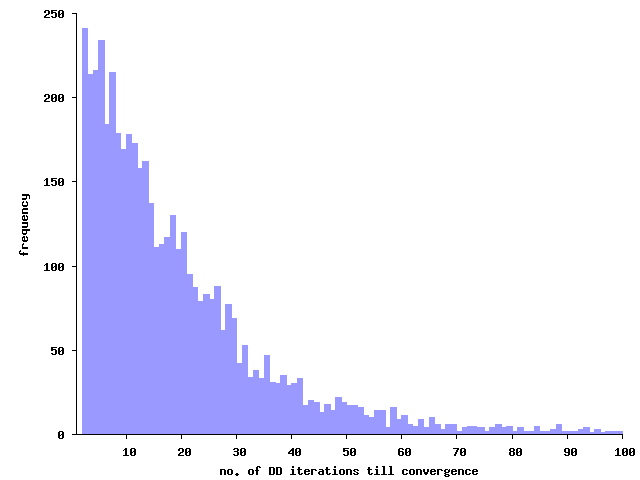
\includegraphics[width=\columnwidth]{histogram.png}
\caption{No. of iterations till DD convergence.}
\label{fig:histo}
\end{center}
\end{figure}



%
%gold: 在 李鄭屋邨 附近
%CRF: 在 李鄭屋邨 附近
%PCT: 在 李鄭屋 邨 附近   <-- DD
%
%gold: 麥 父 笑說
%CRF:  麥 父 笑說
%PCT: 麥父 笑說    <-- DD
%
%gold: 天氣 熱 時 冷氣 大 開     
%CRF: 天氣 熱 時 冷氣 大 開     
%PCT: 天氣 熱時 冷氣 大 開     <-- DD
